% |--- Preâmbulo ---|----------------------{{{
\documentclass[a4paper, 12 pt]{article} % Article são textos pequenos
%\documentclass[a4paper, 12 pt]{report} % Topologia para relatórios
%\documentclass[a4paper, 12 pt]{book} % Livros e Apostilas 
%\documentclass[a4paper, 12 pt]{letter} % Cartas

% |--- Pacotes ---|----------------------{{{

\usepackage[top=1in, bottom=1in, left=1in, right=1in]{geometry} % Margens da Página
\usepackage[utf8]{inputenc} % Codificação do Texto
\usepackage{amsmath, amsfonts, amssymb} % Pacotes de Matemática
\usepackage{graphicx} % Inserir Figuras, gráficos
\usepackage{float} % Inserir figuras: posicionamento
\usepackage[T1]{fontenc}
\usepackage[brazil]{babel} % Para mudar os nomes padrões de comandos
\usepackage{indentfirst} % Sempre identar o 1º parágrafo
\usepackage{ccaption} % Formatas caps de figuras, tabelas
\usepackage{setspace} % Espaçamento Entre Linhas
\usepackage{multicol, multirow} % Mesclar colunas e linhas tabela
\usepackage{fancyhdr} % Personalizar Cabeçalho e Rodapé
\usepackage{enumerate} % Enumerar as páginas
\usepackage{longtable} % Habilitar tabela que é maior que uma página
\usepackage{setspace} % Setar funções de espaço
\usepackage{scalefnt} % Comando \scalefont
\usepackage[final]{pdfpages} % Colocar algum PDF como fundo de página
\usepackage{color, colortbl} % Para usar cor no texto
\usepackage{float}
\usepackage{ifthen}
\usepackage{scalefnt}
\usepackage{graphicx}
\usepackage{hyperref}
\usepackage{subfigure}
\usepackage{enumerate}
\usepackage{caption}
\usepackage[sort,compress]{cite}
\usepackage{natbib} 
\usepackage{booktabs}
\usepackage{comment}
\usepackage{tocbibind}
\usepackage{xcolor}
\usepackage{blindtext}
\usepackage{listings}
\lstset{basicstyle=\ttfamily,
  showstringspaces=false,
  commentstyle=\color{blue},
  keywordstyle=\color{red},
  breaklines=true
}


\renewcommand{\figurename}{Figura}
\renewcommand{\tablename}{Tabela}
\renewcommand{\refname}{Referências}
\newcommand{\sen}{\mathop{\rm sen}}

% Pacotes de Fontes
\usepackage[T1]{fontenc} % Permite que o LaTeX compreenda a acentuação feita direto pelo teclado. É usado com o opcional [T1].
\usepackage{calligra}


\usepackage{color}
\usepackage[normalem]{ulem}
\definecolor{darkgreen}{RGB}{0,80,0}

\newcommand{\old}[1]{{\color{red}\sout{#1}}}
\newcommand{\new}[1]{{\color{blue}#1}}
\newcommand{\commentS}[1]{{\color{darkgreen}{\bfseries [#1]}}}


\title{Trabalho Final}
\author{Danilo Portela de Oliveira \\ danilo.portela@aluno.unb.br}
\date{2022}

\begin{document}

%%%%%%%%%%%CAPA%%%%%%%%%%%%%%%%%%%
	
\thispagestyle{empty}
%\includepdf[pages=1, scale=1.0, frame=false, offset = 0 00, pagecommand={\vspace*{95mm}}]{capa} %% Página Sozinha

\includepdf[pages=1, scale=1.0, frame=false, offset = 0 00, pagecommand=
{\vspace*{35mm}
	\begin{center}
		\scalebox{1.1}{\sffamily{Universidade de Brasília}}\\
		\scalebox{1.1}{\sffamily{Instituto de Geociências - IG}}\\
		%\scalebox{1.1}{\sffamily{Curso}}
		[45pt]
		\scalebox{1.2}{\sffamily{\textbf{Desenvolvimento de metodologia de tomografia sísmica}} }\\[05pt]
		\scalebox{1.2}{\sffamily{\textbf{para aplicações rasas}} }\\[05pt]
		\scalebox{1.2}{ }\\[+35pt]
		\scalebox{1}{Danilo Portela de Oliveira\hspace{05pt}}\\
		\scalebox{1}{}\\[-07pt]
		\scalebox{1}{}\\[20pt]
		\scalebox{1}{Orientador: Marcelo Peres Rocha}\\[10pt]
		\scalebox{1}{Coorientador: Giuliano Sant’Anna Marotta}\\[10pt]
		%\scalebox{1}{}\\[100mm]
		\vfill
		\scalebox{1}{Brasília, XX de Maio de 2022}
\end{center}}]{Figuras/capa_tf.pdf}

\thispagestyle{empty}

\clearpage

%%%%%%%%%%%%%%%% FOLHA DE ROSTO

\begin{center}
	\scalebox{1.1}{\sffamily{Danilo Portela de Oliveira} }\\
	\scalebox{1.1}{\sffamily{} }
	
	\vspace{50mm}
	
	\scalefont{1.5}
	{\sffamily{\textbf{\large{Desenvolvimento de metodologia de tomografia sísmica \\ para aplicações rasas}} }}
	\scalefont{0.67}
	
\end{center}

\vspace{35mm}

\begin{flushright}

\begin{list}{}{
      \setlength{\leftmargin}{8.5cm}
      \setlength{\rightmargin}{0cm}
      \setlength{\labelwidth}{0pt}
      \setlength{\labelsep}{\leftmargin}}

      \item Monografia submetida ao curso de graduação em Geofísica da Universidade de Brasília como requisito para obtenção do Título de Bacharel em Geofísica.
\end{list}
      
\end{flushright}

\begin{center}
	\vspace{15mm}

	Orientador: Marcelo Peres Rocha \\
	Coorientador: Giuliano Sant’Anna Marotta
	
	\vfill
	
	Brasília, XX de Maio de 2022
\end{center}

\clearpage

%%%%%%%%%%%%%%%Agradecimentos%%%%%%%%%%%%%%%%%%%%%%%

\begin{center}
    \large{\textbf{Agradecimentos}}
\end{center}

\blindtext

\blindtext

\blindtext


\clearpage

\clearpage
\hspace{1mm}

\vfill

%%%%%%%%%%%%%%%%%%%%%%%%%%%%%%%%%%%%%%%%%%%%%%

\begin{flushright}
	\begin{itshape}
		``If I have seen further it is by standing on the shoulders of Giants.''\\ Sir Isaac Newton
	\end{itshape}
\end{flushright}

\clearpage

%%%%%%%%%%%%%%%%%%%%%%%%%%%%%%%%%%%%%%%%%%%%%%

\begin{center}
    \large{\textbf{Resumo}}
\end{center}

\blindtext 
%
\blindtext 
%
\blindtext 
%
\blindtext \\

\textbf{Palavras-chave}: \\ \\ ...

\clearpage

%%%%%%%%%%%%%%%%%%%%%%%%%%%%%%%%%%%%%%%%%%%%%%

\begin{center}
    \large{\textbf{Abstract}}
\end{center}

\blindtext 
%
\blindtext 
%
\blindtext 
%
\blindtext \\
\\
\\
\\
\textbf{Keywords}:
\\
\\
...



\clearpage

\begin{center}
\listoffigures \newpage % Plotar a lista de figuras
\end{center}

\begin{center}
\listoftables \newpage % Plotar a lista de tabelas
\end{center}

\begin{center}
    \large{\textbf{Lista de Símbolos}}
\end{center}

\vspace{0.5cm}

\begin{comment}
$V_{p}$ - Velocidade da onda sísmica P

\vspace{0.5cm}

$V_{s}$  - Velocidade da onda sísmica S

\vspace{0.5cm}

$k$ - Módulo de compressibilidade

\vspace{0.5cm}

$\mu$ - Módulo de cisalhamento

\vspace{0.5cm}

$\rho$ - Densidade do meio

\vspace{0.5cm}

$\sigma$ - Razão de Poisson

\vspace{0.5cm}

$\lambda$ - Primeiro coeficiente de Lamé

\vspace{0.5cm}

$\delta$ - Delta de Dirac

\vspace{0.5cm}

$\ast$ - Convolução

\vspace{0.5cm}

$\otimes$ - Correlação

\vspace{0.5cm}


$G$ - Função de Green

\vspace{0.5cm}

$f_{p}$ - Frequência de pico

\vspace{0.5cm}

$g_{2}$ - 2$^{a}$ Derivada da Gaussiana (Ricker)

\vspace{0.5cm}

$tmod$ - Tempo total de gravação 

\vspace{0.5cm}

MWCS - \emph{Moving Window Cross Spectral}
\end{comment}

\clearpage

%%%%%%%%%%%%%%%%%%%%%%%%%%%%%%%%%%%%%%%%%%%%%%%%%%%%

\begin{center}
\tableofcontents \newpage % Plotar o sumário
\end{center}

\clearpage

%%%%%%%%%%%%%%%%%%%%%%%%%%%%%%%%%%%%%%%%%%%%%%

\section[Introdução]{Introdução}


\blindtext 
%
\blindtext 
%
\blindtext 
%
\blindtext

%%%%%

\clearpage

%%%%%%%%%%%%%%%%%%%%%%%%%%%%%%%%%%%%%%%%%%%%%%%%%

\section{Fundamentação Teórica}

\subsection{Formulando problemas inversos}

O ponto de partida na maioria dos problemas inversos é uma descrição dos dados. Como na maioria dos problemas inversos os dados são simplesmente uma tabela de valores numéricos, um vetor fornece um meio conveniente de sua representação \citep{menke1984geophysical}.

Se as medições $N$ forem realizadas em um experimento específico, por exemplo, pode-se considerar esses números como os elementos de um vetor $\textbf{d}$ de comprimento $N$. Da mesma forma, os parâmetros do modelo podem ser representados como os elementos de um vetor $\textbf{m}$, que é de comprimento $M$.

\begin{equation}\label{eq:tomography}
\begin{split}
\textrm{dados}: \textbf{d} &= [d_{1}, d_{2}, d_{3}, d_{4}, \dots, d_{N}]^T \\
\textrm{parâmetros do modelo}: \textbf{m} &= [m_{1}, m_{2}, m_{3}, m_{4}, \dots, m_{N}]^T
\end{split}
\end{equation}

Aqui $T$ significa a matriz transposta. 

A afirmação básica de um problema inverso é que os parâmetros do modelo e os dados estão de alguma forma relacionados. Essa relação é chamada de \textit{modelo}. Normalmente, o modelo assume a forma de uma ou mais fórmulas que os dados e os parâmetros do modelo devem seguir.

Se, por exemplo, alguém estivesse tentando determinar a densidade de um objeto medindo sua massa e volume, haveria dois dados - massa e volume (digamos, $d_{1}$ e $d_{2}$, respectivamente) - e um parâmetro de modelo desconhecido, densidade (digamos, $m_{1}$). O modelo seria a afirmação de que densidade vezes volume é igual a massa, o que pode ser escrito de forma compacta pela equação vetorial $d_{2}m_{1} = d_{1}$.

Em situações mais realistas, os dados e os parâmetros do modelo são relacionados de maneiras mais complicadas. Mais geralmente, os dados e os parâmetros do modelo podem estar relacionados por uma ou mais equações implícitas, como

\begin{equation}\label{eq:formulation}
\begin{matrix}
f_{1}(\textbf{d, m}) &=& 0 \\
f_{2}(\textbf{d, m}) &=& 0 \\
&\vdots \\
f_{L}(\textbf{d, m}) &=& 0 \\
\end{matrix}
\end{equation}

Onde $L$ é o número de equações. As Equações em  ~(\ref{eq:formulation}) da página~\pageref{eq:formulation} relativos à medição de densidade, $L = 1$ e $d_{2}m_{1} = d_{1}$ constituiria a única equação da forma $f_{1}(\textbf{d, m}) = 0$. Essas equações implícitas, que podem ser escritas de forma compacta como a equação vetorial $\textbf{f(d, m)} = 0$, resume o que se sabe sobre como os dados medidos e os parâmetros desconhecidos do modelo estão relacionados. O propósito da teoria inversa é resolver, ou ``inverter'', essas equações para os parâmetros do modelo, ou quaisquer tipos de respostas que possam ser possíveis ou desejáveis em qualquer situação.

Nenhuma afirmação é feita de que as equações $\textbf{f(d, m)} = 0$ contenham informações suficientes para especificar os parâmetros do modelo de forma única ou que sejam consistentes. Um dos propósitos da teoria inversa é responder a esses tipos de perguntas e fornecer meios de lidar com os problemas que elas implicam. Em geral, $\textbf{f(d, m)} = 0$ pode consistir em funções arbitrariamente complicadas (não lineares) dos dados e parâmetros do modelo. Em muitos problemas, no entanto, a equação assume uma das várias formas simples.

\subsubsection{Forma linear implícita}

A função $\textbf{f}$ é linear em ambos os parâmetros de dados e modelo e, portanto, pode ser escrita como a equação matricial (Equações em~(\ref{eq:formulation}) da página~\pageref{eq:formulation}). O Problema Linear Inverso

\begin{equation}\label{eq:matriz}
\textbf{f(d, m)} = 0 = \textbf{F}
\begin{bmatrix}
\textbf{d} \\
\textbf{m}
\end{bmatrix}
\end{equation}
onde $\textbf{F}$ é uma matriz $L \times (M + N)$.

\subsubsection{Forma explícita}

Em muitos casos, é possível separar os dados dos parâmetros do modelo e, assim, formar $L = N$ equações que são lineares nos dados (mas ainda não lineares nos parâmetros do modelo por meio de uma função vetorial $\textbf{g}$).

\begin{equation}\label{eq:forma_explicita}
\textbf{f(d, m)} = 0 = \textbf{d} - \textbf{g(m)}
\end{equation}

\subsubsection{Forma linear explícita}

Na forma linear explícita, a função $\textbf{g}$ também é linear, levando à equação matricial $N \times M$ (onde $L = N$)

\begin{equation}\label{eq:forma_linear_explicita}
\textbf{f(d, m)} = 0 = \textbf{d} - \textbf{Gm}
\end{equation}

Usar esta forma é equivalente a dizer que a matriz $\textbf{F}$ na Seção 2.1.1 é uma matriz diagonal.

\begin{equation}\label{eq:matriz_linear}
\textbf{F} = 
\begin{bmatrix}
\textbf{-I} & \textbf{0}\\
\textbf{0}	&	\textbf{G}
\end{bmatrix}
\end{equation}

%%%%%%%%%%%%%%%%%%%%%%%%%%%%%%%%%%%%%%%%%%%%%%

\subsubsection{Exemplos de formulação de problemas inversos}

\begin{description}
	\item[Exemplo 1] |\textit{Ajustando uma linha reta} 
\end{description}

Suponha que $N$ medições de temperatura $T_{i}$ sejam feitas em profundidades $z_{i}$ na terra \citep{menke1984geophysical}. Os dados então são, um vetor $\textbf{d}$ de $N$ medições de
temperatura, onde $\textbf{d} = [T_{1}, T_{2}, T_{3}, \cdots, T_{N}]^T$. As profundidades $z_{i}$, não são, estritamente falando, dados. Em vez disso, eles fornecem algumas informações auxiliares que descrevem a geometria do experimento. Essa distinção será melhor esclarecida a seguir.

Suponha que assumimos um modelo no qual a temperatura é uma função linear da profundidade: $T = a + bz$. O coeficiente linear $a$ e o coeficiente angular $b$ formam então os dois parâmetros do modelo do problema, $\textbf{m} = [a, b]^T$. De acordo com o modelo, cada observação de temperatura deve satisfazer $T = a + bz$: 

\begin{equation}\label{eq:formulation_tem}
\begin{matrix}
T_{1} &=& a + bz_{1} \\
T_{2} &=& a + bz_{2} \\
&\vdots \\
T_{N} &=& a + bz_{N} \\
\end{matrix}
\end{equation}

Essas equações~(\ref{eq:formulation_tem}), página~\pageref{eq:formulation_tem}, podem ser organizadas como a equação matricial $\textbf{Gm = d}$: \\

\begin{equation}\label{eq:matriz_temperatura}
\begin{bmatrix}
T_{1} \\
T_{2} \\
\vdots \\
T_{N}\\
\end{bmatrix} = 
\begin{bmatrix}
1 & z_{1} \\
1 &	z_{2} \\
\vdots & \vdots \\
1 & z_{N} \\
\end{bmatrix}
\begin{bmatrix}
a \\
b \\
\end{bmatrix}
\end{equation} \\

\begin{description}
	\item[Exemplo 2] |\textit{Tomografia acústica} 
\end{description}

Suponha que uma parede seja montada a partir de um arranjo retangular de tijolos~(Figura \ref{tomografia}, página~\pageref{tomografia}) e que cada tijolo seja composto de um tipo diferente de argila \citep{menke1984geophysical}. Se as velocidades acústicas das diferentes argilas diferem, pode-se tentar distinguir os diferentes tipos de tijolos medindo o tempo de viagem do som através das várias fileiras e colunas de tijolos na parede. Os dados deste problema são $N = 8$ medições de tempo de percurso, $\textbf{d} = [T_{1}, T_{2}, T_{3}, \cdots, T_{8}]^T$. 

O modelo assume que cada tijolo é composto de um material uniforme e que o tempo de percurso do som através de cada tijolo é proporcional à largura e altura do tijolo. O fator de proporcionalidade é a lentidão (\textit{slowness}) do tijolo $s_{i}$, dando assim $M = 16$ parâmetros do modelo $\textbf{m} = [s_{1}, s_{2}, s_{3}, \cdots, s_{16}]^T$, onde a ordenação está de acordo com o esquema de numeração da figura como \\


\begin{equation}\label{eq:formulation_tomografia}
\begin{matrix}
Linha 1: T_{1} &=& hs_{1} + hs_{2} + hs_{3} + hs_{4} \\
Linha 2: T_{2} &=& hs_{5} + hs_{6} + hs_{7} + hs_{8} \\
&\vdots \\
Coluna 4: T_{8} &=& hs_{4} + hs_{8} + hs_{12} + hs_{16} \\
\end{matrix}
\end{equation} \\
e a equação matricial é \\

\begin{equation}\label{eq:matriz_tomografia}
\begin{bmatrix}
T_{1} \\
T_{2} \\
\vdots \\
T_{8}\\
\end{bmatrix} = h \left[
\begin{array}{cccccccccccccccc}
1 & 1 & 1 & 1 & 0 & 0 & 0 & 0 & 0 & 0 & 0 & 0 & 0 & 0 & 0 & 0 \\
0 & 0 & 0 & 0 & 1 & 1 & 1 & 1 & 0 & 0 & 0 & 0 & 0 & 0 & 0 & 0 \\
\vdots & \vdots & \vdots & \vdots & \vdots & \vdots & \vdots & \vdots & \vdots & \vdots & \vdots & \vdots & \vdots & \vdots & \vdots & \vdots \\
0 & 0 & 0 & 1 & 0 & 0 & 0 & 1 & 0 & 0 & 0 & 1 & 0 & 0 & 0 & 1 \\
\end{array}\right]
\begin{bmatrix}
s_{1} \\
s_{2} \\
\vdots \\
s_{16}\\
\end{bmatrix}
\end{equation}

\begin{figure}[!hbtp]
	\begin{center}
		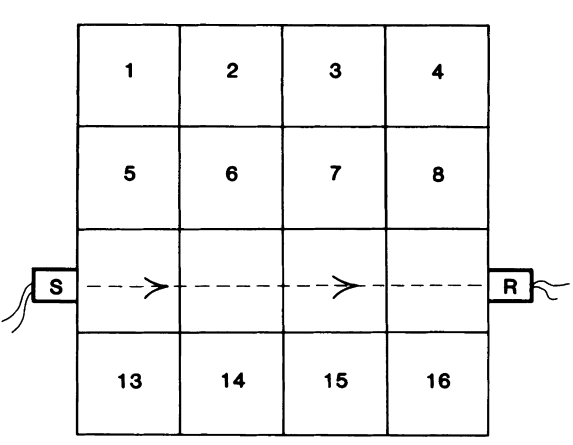
\includegraphics[scale=0.45]{Figuras/tomografia.png}
	\end{center}
	\caption{O tempo de percurso das ondas acústicas (linhas tracejadas) através das linhas e colunas de uma matriz quadrada de tijolos é medido com a fonte acústica $\textbf{S}$ e o receptor $\textbf{R}$ colocados nas bordas do quadrado. O problema inverso é inferir as propriedades acústicas dos tijolos (que são assumidas como homogêneas). \cite{menke1984geophysical}.}
	\label{tomografia}
\end{figure}

\newpage
%%%%%%%%%%%%%%%%%%%%%%%%%%%%%%%%%%%%%%%%%%%%%%

\subsection{O Problema Linear Inverso}

Os problemas inversos mais simples e mais bem compreendidos são aqueles que podem ser representados com a equação linear explícita $\textbf{Gm = d}$. Esta equação, portanto, forma a base do estudo da teoria inversa discreta. Muitos problemas inversos importantes que surgem nas ciências físicas envolvem precisamente essa equação. Outros, embora envolvam equações mais complicadas, muitas vezes podem ser resolvidos por meio de aproximações lineares.

A matriz $\textbf{G}$ é chamada de \textit{data kernel}, em analogia à teoria das equações integrais, na qual os análogos aos vetores de parâmetros de dados e modelos são duas funções contínuas $d(x)$ e $m(x)$, onde $x$ é alguma variável independente. As duas funções estão relacionadas pela equação

\begin{equation}\label{eq:inversão}
d(x) = \int G(x, \xi)m(\xi)d\xi
\end{equation}
onde a função $G(x, \xi)$ é o \textit{kernel}, ou função de Green, da equação integral. A solução de problemas desse tipo está dentro do escopo da teoria inversa contínua.

%%%%%%%%%%%%%%%%%%%%%%%%%%%%%%%%%%%%%%%%%%%%%%

\subsection{Tomografia}

O objetivo basal da Geofísica é obter informações a cerca dos parâmetros físicos das rochas que constituem o interior da Terra a partir de dados medidos em superfície, em poços ou em levantamentos aéreos \citep{reis2015aplicaccao}. Na modelagem direta, aplicam-se as equações que descrevem as leis da física sobre um modelo previamente definido para a obtenção de dados de resposta referentes aos parâmetros físicos desse tal modelo. Em contra partida, no problema inverso, já se possui os dados de resposta, aqueles obtidos através de levantamentos, e, portanto, o objetivo agora é a estimativa de um modelo que, quando aplicado a uma determinada relação físico-matemática, melhor se adéque aos dados medidos.

A tomografia sísmica é uma metodologia de inferência de parâmetros numéricos, usada na Geofísica, que extrai informações contidas em registros sísmicos para estimar modelos bidimensionais ou tridimensionais do interior da Terra \citep{rawlinson2010seismic}. Em geral, requer a solução de um problema inverso para se obter um modelo de velocidades sísmicas que seja consistente com as observações de campo. Desde que seja possível estabelecer um modelo aproximado $\textbf{d} = g(\textbf{m})$ , entre o vetor de dados sísmicos $\textbf{d}$ e o vetor de parâmetros do modelo sísmico $\textbf{m}$ - de modo que, para um dado modelo $\textbf{m}$, seja possível prever $\textbf{d}$ - procura-se, na tomografia sísmica, encontrar $\textbf{m}$ tal que $\textbf{d}_{obs} = g(\textbf{m})$, onde $\textbf{d}_{obs}$ é o vetor de dados observados.

As relações do tipo $\textbf{d} = g(\textbf{m})$, em sua grande maioria, são não-lineares e não solucionáveis analiticamente \citep{reis2015aplicaccao}, por isso, busca-se a linearização dessas relações através de
métodos numéricos. Com isso, devido a essa não-linearidade do problema inverso, a superfície da função-objetivo dos tempos de percurso pode não vir a ser simples, bem comportada ou com um único mínimo bem definido. 

Devido, também, ao caráter discreto dos dados geofísicos, faz-se necessário o uso de uma formulação matricial para o tratamento desses dados \citep{reis2015aplicaccao}. O objetivo agora, então, é criar uma aproximação linearizada $\textbf{Gm = d}$, onde $\textbf{d}$ é um vetor p-dimensional que carrega os dados medidos nos levantamentos, $\textbf{m}$ é um vetor n-dimensional que carrega os parâmetros do modelo o qual se quer estimar a partir das medidas, e $\textbf{G}$ é uma matriz de dimensões $\textit{p}$ por $\textit{n}$ que, se inversível, nos levaria facilmente a solução do problema através da relação $\textbf{m} = \textbf{G}^{-1}\textbf{d}$. Todavia, na quase totalidade dos problemas geofísicos, os problemas são
mal postos \citep{reis2015aplicaccao}, ou seja, não obedecem aos critérios de existência, unicidade e estabilidade simultaneamente; e $\textbf{Gm = d}$ constitui-se num sistema sobredeterminado $(\textit{m} > \textit{n})$, onde $\textbf{G}$ não é, à rigor, inversível; e, portanto, se faz necessário o uso de métodos numéricos mais complexos e, também, a consulta de informações geológicas à priori que, de alguma forma, limite os graus de liberdade do problema.

A tomografia sísmica possui grande importância no processamento sísmico. Através dela, é possível extrair diversas informações dos registros sísmicos, os quais se incluem tempos de percurso, amplitudes, conteúdo de frequências ou, até mesmo, a forma total da onda. Ela pode ser considerada, por exemplo, um complemento natural para a migração sísmica, pois oferece um meio de estimar a velocidade e a profundidade de interfaces usando tempos de percurso e, com menos frequência, amplitudes de espalhamento geométrico e coeficientes de reflexão/transmissão \citep{reis2015aplicaccao}.

\subsubsection{Tomografia sísmica por tempo de percurso}

A inversão sísmica de tempo de percurso para a estrutura de velocidades é um problema não linear, uma vez que os raios sísmicos, atuando como caminhos integrais em uma inversão tomográfica, dependem também da velocidade média (\citealp{worthington1984introduction}; \citealp{zhou2003crosshole}). Em vez de determinar os caminhos de raios desconhecidos e a estrutura de velocidade desconhecida simultaneamente, muitas vezes usa-se uma solução linearizada de forma iterativa para resolver as perturbações do modelo, em vez dos parâmetros do modelo diretamente \citep{bording1987applications}. As perturbações do modelo são consideradas pequenas o suficiente para que se possa considerar a relação entre as perturbações do modelo e os resíduos correspondentes como linear. Uma vez que as perturbações do modelo tenham sido encontradas, elas são adicionadas ao modelo atual para produzir o modelo para a iteração seguinte até que o resultado convirja.

Na prática, os dados sísmicos às vezes contêm uma quantidade considerável de ruído. Para dados de tempo de percurso, a precisão de leitura finita é a principal fonte de erros de dados. Para reduzir os erros, um método de pré-processamento é calcular a média dos dados de tempo de percurso de caminhos de raios semelhantes \cite{rohm2000effects}, mas esse método pode funcionar apenas em tomografia telessísmica, pois os erros são relativamente pequenos em comparação com os dados reais do tempo de percurso. Para mitigar os erros de dados, \cite{wang2000seismic} separaram os dados de tempo de percurso com ruído usando uma regressão ponderada localmente para se livrar dos valores discrepantes ou reduzir o peso dos grandes erros de separação. Para reduzir o efeito de erros de dados durante a inversão, \cite{scales1988fast} usaram coeficientes de ponderação em função do tempo de percurso residual em um esquema de mínimos quadrados iterativamente reponderado. Esses pesos baseados em resíduos, no entanto, são subjetivos, uma vez que os erros de dados na prática podem ter uma distribuição não Gaussiana e, portanto, o resíduo de dados pode ser enviesado. \cite{cao1995relative} montaram um esquema de inversão não linear baseado em erro relativo para dados sísmicos de \textit{crosshole} que tenta superar o viés dos métodos de mínimos quadrados que tendem a enfatizar raios com maiores tempos de percurso.

\subsubsection{Reconstrução na tomografia sísmica de tempo de percurso}

O problema de reconstruir imagens por projeções, isto é, reconstruir uma função através de suas integrais ao longo de retas surgiu independentemente em diversos ramos da ciência tais como na Geofísica, Astrofísica, Medicina e dentre
outros. 

Provavelmente os exemplos que causaram maior impacto na vida moderna foram em prospecção sísmica e na tomografia computadorizada voltada para diagnósticos clínicos.

O termo tomografia surge do prefixo grego ``tomo'' que quer dizer fatia, o que nos sugere uma reconstrução em 2-D. Mas a palavra já é utilizada rotineiramente para se referir a reconstrução de imagens em 3-D, sobretudo pelos sismólogos e radiólogos.

A tomografia sísmica tem como preocupação, a reconstrução de imagens de estruturas em subsuperfície. Dentre as técnicas existentes focalizaremos a que utiliza dados de tempo de percurso \citep{tempopercurso}.

Iniciaremos com a descrição do Princípio de Fermat. Neste contexto, é natural introduzir a vagarosidade, ou seja, a inversa da velocidade.

Dada $s$ uma distribuição contínua da vagarosidade $s(x)$, \textit{o tempo de percurso} de um sinal ao longo de um possível caminho que liga a fonte que o emitiu ao receptor é dado pela Equação~(\ref{eq:tempo_percurso}) da página~\pageref{eq:tempo_percurso}:

%%%%%%%%%%%%%%%%Início - Equação%%%%%%%%%%%%%%%%%%%%%%

\begin{equation}\label{eq:tempo_percurso}
\tau^p(s) = \int_P s(x) \, dl^P = \int_P \frac{1}{v(x)} \, dl^P
\end{equation}

%%%%%%%%%%%%%%%%Fim - Equação%%%%%%%%%%%%%%%%%%%%%%%%%

Onde $dl^P$ denota o comprimento de arco ao longo do caminho $P$. Denotemos por $\tau$ o conjunto de todos os possíveis caminhos ligando a fonte ao receptor.

O Princípio de Fermat diz que o caminho físico percorrido por uma onda entre dois pontos é aquele que minimiza o tempo de percurso.

%%%%%%%%%%%%%%%%Início - Equação%%%%%%%%%%%%%%%%%%%%%%

\begin{equation}\label{eq:tempo_min}
\tau^*(s) = min_{P \in \{\tau\}} \tau^P (s)
\end{equation}

%%%%%%%%%%%%%%%%Fim - Equação%%%%%%%%%%%%%%%%%%%%%%%%%

O funcional $P \mapsto \tau^p(s)$ de tempo de percurso é estacionário com respeito a pequenas pertubações no caminho de Fermat $P^*(s)$ no sentido do cálculo das variações \citep{Axelsson}. Observe que a Equação~(\ref{eq:tempo_min}) da página~\pageref{eq:tempo_min} depende de forma não linear em \textit{s}, como consequência do processo de minimização.

Uma forma de obter dados na tomografia sísmica é feita aproveitando a existência de poços já perfurados. Isto é, colocando transmissores em um dos poços e receptores em outro de maneira que são emitidas ondas entre os poços.
Tais ondas podem ser sísmicas ou eletromagnéticas. Através da utilização de receptores apropriados mede-se o tempo de chegada das mesmas.

Esses dados, apesar de imprecisos e ruidosos, podem ser utilizados para obtermos informações sobre a composição do subsolo e a presença de hidro-carbonetos.

%%%%%%%%%%%%%%%%%%%%%%%%%%%%%%%%%%%%%%%%%%%%%%%%

\subsubsection{Problema Direto}

Dentro de uma aproximação aceitável para muitas finalidades em Geofísica, podemos modelar as ondas sísmicas como soluções da equação diferencial parcial:

\begin{equation}\label{eq:problema_direto}
\partial_{t}^2 \phi - c^2(x)  \Delta \phi = g(x, t)
\end{equation}
onde $g(x, t)$ é a intensidade da pertubação num determinado ponto $x$ e tempo $t$. Temos que $\phi (x, t)$ é a intensidade da onda no tempo $t$ e posição $x$. Esta equação deve ser complementada com condições de contorno apropriadas.

O problema direto consiste em resolver a equação dado $g$, isto é, encontrar a solução $\phi$. No caso da tomografia por tempo de percurso, a preocupação é determinar o tempo de percurso da frente de onda e o caminho percorrido pela mesma entre fonte e receptor. Para saber mais sobre as técnicas de resolução desse tipo de problema direto ver \citep{rawlison}.

%%%%%%%%%%%%%%%%%%%%%%%%%%%%%%%%%%%%%%%%%%%%%%

\subsubsection{Problema Inverso}

Para o problema inverso~(Figura \ref{direto_inverso}\textbf{a}, página~\pageref{direto_inverso}), queremos obter informações sobre os coeficientes da equação utilizando dados sobre suas soluções em regiões distintas. As técnicas de problemas inversos são de grande interesse na prospecção sísmica, pois têm por objetivo, determinar o interior da região em estudo somente com base em informação parcial dos dados no exterior da mesma. Assim, nos propomos a reconstruir os valores de $c(x)$ com base na solução da
equação da onda medida na fronteira que delimita a região de interesse. Com essas informações em mãos, os geólogos e geofísicos podem inferir que tipo de material existe no subsolo estudado fazendo uso de informações como por
exemplo na Figura~\ref{material} (página~\pageref{material}).

Na inversão linear na tomografia por tempo de percurso, assumimos à priori que sabemos o traçado dos feixes que ligam fonte a receptor, o que é justificado por uma aproximação linear que ignora a dependência que os caminhos possuem da distribuição da vagarosidade (Princípio de Fermat).

Na~Figura \ref{direto_inverso}\textbf{a} (página~\pageref{direto_inverso}) descrevemos simplificadamente uma comparação entre o problema direto e o problema inverso. O problema inverso é relativamente mais complicado, uma vez que, em problemas reais, fixados os dados, podemos construir infinitos modelos que se adéquam a estes mesmos dados. No problema inverso, muitas vezes não há essa unicidade levando dos dados ao modelo. Assim, chegamos a um esquema mais adequado à realidade na Figura~\ref{direto_inverso}\textbf{b} (página~\pageref{direto_inverso}).

A não unicidade do problema inverso pode ser explicada pelo fato de possuirmos somente uma quantidade finita de dados coletados para obter um modelo que muitas vezes é uma função contínua de suas variáveis, o que significa, que o mesmo possui infinitos graus de liberdade. Por causa dessa limitação física da finitude dos dados, o modelo que alcançamos através dos dados coletados não é necessariamente o que modela a realidade.

São necessários dois passos na inversão para chegarmos a um modelo mais próximo da realidade. Isto é representado na Figura~\ref{direto_inverso}\textbf{b} (página~\pageref{direto_inverso}). Vale salientar que em última análise o modelo verdadeiro não é sabido em problemas reais.

O primeiro passo seria então reconstruir um modelo $m'$ utilizando os dados $d$. Uma vez feito isto, determinamos que propriedades o modelo $m'$ preserva do modelo real $m$ e que tipo de erros e ruídos estão associados a ele, ou seja,
fazemos uma avaliação do modelo.

\begin{figure}[!hbtp]
	\begin{center}
		
		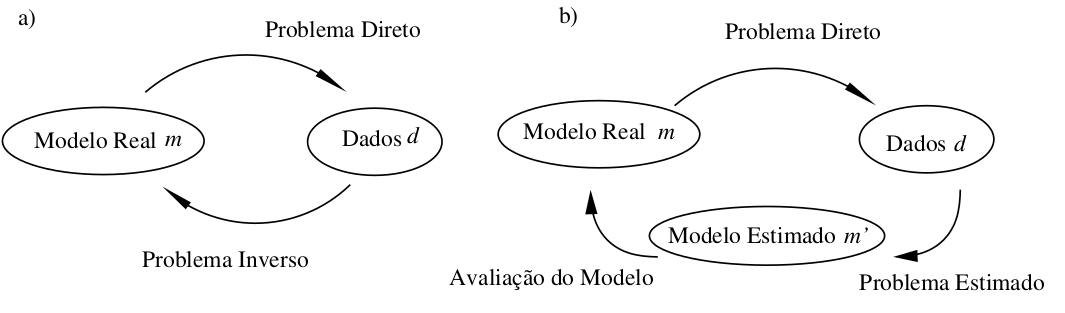
\includegraphics[scale=0.43]{Figuras/problema_direto_x_inverso.png}
	\end{center}
	\caption{(a) Problema Direto versus Problema Inverso. (b) O problema inverso visto com duas etapas. \cite{tempopercurso}.}
	\label{direto_inverso}
\end{figure}

\begin{figure}[!hbtp]
	\begin{center}
		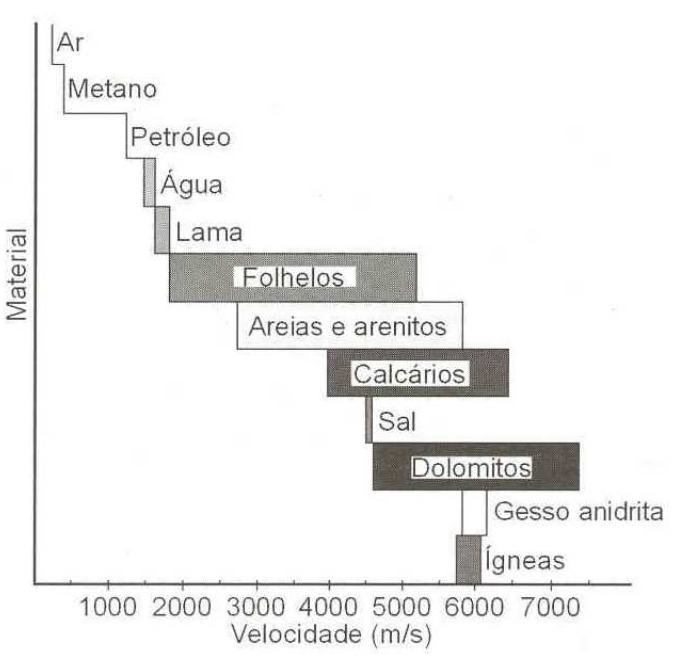
\includegraphics[scale=0.32]{Figuras/material.png}
	\end{center}
	\caption{Gráfico de materiais de acordo com a velocidade. Assim, com a solução obtida pela tomografia de tempo de percurso, os geólogos e geofísicos podem inferir que tipo de material existe no subsolo. \cite{tempopercurso}.}
	\label{material}
\end{figure}

\newpage

%%%%%%%%%%%%%%%%%%%%%%%%%%%%%%%%%%%%%%%%%%%%%%

\subsection{Modelos (Representação da Estrutura)}

Mostraremos duas maneiras de parametrizar a vagarosidade \citep{tempopercurso}. O mais simples seria dividir a região em pequenos blocos (denominados pixels no caso 2-D e voxels no caso 3-D) e atribuir valores constantes à vagarosidade em cada bloco. Isto pode ser visto na Figura~\ref{modelos}\textbf{a} (página~\pageref{modelos}). 

Uma alternativa a este modelo é definir vagarosidade nos vértices da malha formada pela divisão da região em blocos (Figura~\ref{modelos}\textbf{b}, página~\pageref{modelos}). Essa definição seria
formulada em conjunto com uma função de interpolação. Um exemplo ilustrativo disto seria no contexto de tomografia local de terremotos, tal que para cada vértice $(x, y, z)$ é utilizada uma interpolação trilinear (figura~\ref{modelos}\textbf{c}, página~\pageref{modelos}):

\begin{figure}[!hbtp]
	\begin{center}
		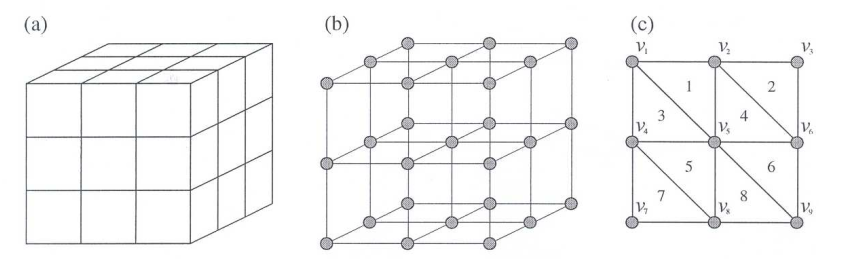
\includegraphics[scale=0.50]{Figuras/modelos.png}
	\end{center}
	\caption{Modelos. \cite{tempopercurso}.}
	\label{modelos}
\end{figure}

\begin{equation}\label{eq:estrutura}
v(x, y, z) = \sum_{i=1}^{2} \sum_{j=1}^{2} \sum_{k=1}^{2} V(x_{i}, y_{j}, z_{k})\left(1 - \left|\frac{x - x_{i}}{x_{2} - x_{1}}\right|\right)\left(1 - \left|\frac{y - y_{j}}{y_{2} - y_{1}}\right|\right)\left(1 - \left|\frac{z - z_{k}}{z_{2} - z_{1}}\right|\right)
\end{equation} \\
onde $V(x_{i}, y_{j}, z_{k})$ são os valores da velocidade nos oito vértices que cercam o vértice $(x, y, z)$.


Para este trabalho estamos interessados em entender o primeiro modelo acima (Figura~\ref{modelos}\textbf{a}, página~\pageref{modelos}). Sendo assim, considere $t_{1}, \cdots, t_{m}$ conjunto de tempos de percurso entre fonte e receptor. Dado um modelo com n células, podemos escrever, 

\begin{equation}\label{eq:percurso}
t_{i} = \sum_{j=1}^{n} l_{ij}s_{j},
\end{equation}

\begin{figure}[!hbtp]
	\begin{center}
		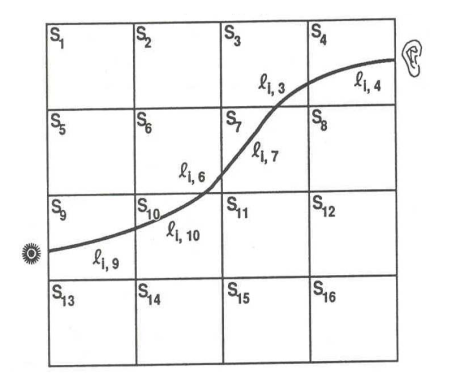
\includegraphics[scale=0.60]{Figuras/tempo_percurso.png}
	\end{center}
	\caption{Tempo de percurso para a $i$-ésima frente de onda, onde está sendo utilizado o modelo discretizado com vagarosidade constante em cada pixel. \cite{tempopercurso}.}
	\label{modelos_percurso}
\end{figure} \newpage
Ou melhor,  $Ms = t$. Onde $M$ é a matriz formada pelo comprimento $l_{ij}$ do $i$-ésimo raio que passa pela $j$-ésima célula e $s$ é a vagarosidade (a nossa incógnita). Observe que

\begin{equation}\label{eq:percurso_comprimento}
l_{ij} = \frac{\partial t_{i}}{\partial s_{j}}
\end{equation}
e assim,

\begin{equation}\label{eq:percurso_comprimento2}
t_{i} = \frac{\partial t_{i}}{\partial s_{1}}s_{1} + \frac{\partial t_{i}}{\partial s_{2}}s_{2} + \cdots + \frac{\partial t_{i}}{\partial s_{n}}s_{n}.
\end{equation}
\\

Assim, discretizando o domínio da vagarosidade obtemos um sistema de equações lineares, onde a matriz do sistema é muito esparsa (A densidade de uma matriz é o número de elementos não nulos dividido pelo total de elementos da matriz. Se esse número for muito pequeno essa matriz é dita esparsa) porque cada raio intersecta somente uma pequena fração dos voxels da discretização (ver Figura~\ref{modelos_percurso}, página~\pageref{modelos_percurso}). Então para os pixels em 2-D, cada raio intersecta algo da ordem de $m * n$ pixels em uma malha $m \times n$. Isso torna o problema particularmente atrativo para a utilização de soluções iterativas. 

A matriz $M$ contém todas as informações físicas e matemáticas que escolhemos para o modelo no problema dado. Assim, no caso da tomografia por tempo de percurso, a matriz
$M$ terá como suas componentes os dados do comprimento das trajetórias.

\begin{figure}[!hbtp]
	\begin{center}
		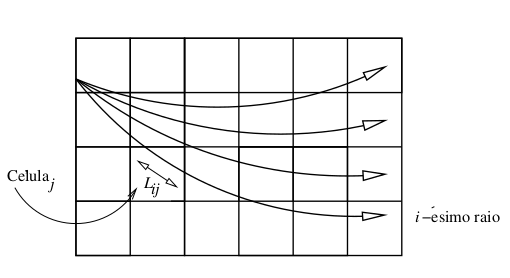
\includegraphics[scale=0.60]{Figuras/diagrama.png}
	\end{center}
	\caption{Diagrama de um experimento tomográfico. A matriz $M$ geralmente é esparsa, pois existem células por onde não passam nenhum raio do experimento. \cite{tempopercurso}.}
	\label{modelos_diagrama}
\end{figure} \newpage

%%%%%%%%%%%%%%%%%%%%%%%%%%%%%%%%%%%%%%%%%%%%%%

\subsection{Matriz de percurso dos raios}

As entradas em $\textbf{S}$ (Figura~\ref{matriz_convergencia}, página~\pageref{matriz_convergencia}) são calculadas identificando a interseção de forma individual do raio \textit{`m'} com os limites do pixel \textit{`n'} e computando o comprimento (relação de Pitágoras) \textit{`d'} dentro do elemento \citep{RBGf1495}. Portanto, o tamanho de $\textbf{S}$ crescerá com o incremento das medidas e/ou densidade de discretização.

Considerando a Figura~\ref{raios} (página~\pageref{raios}) e tendo ainda em mente a Figura~\ref{matriz_convergencia} (página~\pageref{matriz_convergencia}); o número de fontes e receptores é $7$ e então o número total de raios é $49$ (constante para esta matriz). Se o meio for dividido em $7 \times 7 = 49$ pixels, $\textbf{S}$ será de 49 linhas ($M$, número de raios) por 49 colunas ($N$ , número de pixels, cujas lentidão (\textit{slowness}) são desconhecidas). É relevante notar que o incremento da densidade de pixels $(N)$, levará a considerar mais pixels no cálculo dos caminhos de viagem para cada receptor.

Este sistema de equações é \textit{aparentemente} determinado (número de equações igual ao número de incógnitas). A palavra \textit{aparentemente} significa que em alguns casos (especialmente em \textit{cross-hole}, (ver \citealp{imhof2007caracterizacion}) o sistema está mal condicionado e a classificação de $\textbf{S} < N , M$. Isso dará um sistema subdeterminado levando a infinitas soluções. O mesmo ocorrerá, por exemplo, dividindo o meio em mais pixels para melhorar a resolução das imagens. (a limitação de dividir o meio com $N = M$ é que a resolução é grosseira, pois o tamanho dos pixels é grande).

Incrementar o número de transdutores para melhorar a resolução não é prático e sempre possível; primeiro, devido à quantidade de esforço de levantamento necessário (custo) e, segundo, se os raios estão tão próximos, a condição de matriz S aumenta e não necessariamente adiciona informações ao sistema (\citealp{santamarina1998introduction}; \citealp{fernandez2000tomographic}).

%%%%%%%%%%%%%%%%%%%%%%%%%%%%%%%%%%%%%%%%%%%%%%

\subsection{Matriz de cobertura espacial}

O tamanho de $\textbf{S}$ (matriz de transformação) é $M$ linhas (número de medições) por $N$ colunas (número de lentidão - \textit{slowness} - de pixel desconhecido). A soma de cada coluna individual de $\textbf{S}$ traz o comprimento total percorrido pelos raios em um pixel (Figura~\ref{matriz_convergencia}, página~\pageref{matriz_convergencia}). Aplicando esta soma em todas as colunas de $\textbf{S}$, obtém-se um vetor linha $1 \times N$ que rearranjado seguindo o padrão geométrico, traz a matriz de cobertura espacial de $``s"$ pixels verticais por $``t"$ horizontais onde $N = s + t$. Considerou-se aqui $s = t$ \citep{RBGf1495}.

Dois exemplos de matrizes de cobertura espacial de \textit{cross-hole} são representados na Figura~\ref{raios_convergencia} (página~\pageref{raios_convergencia}) para 10 pares de fonte-receptor; \textbf{(a)} para 100 elementos e \textbf{(b)} 400 unidades. As zonas escuras indicam valores mais baixos de cobertura espacial. Isso significa que as informações coletadas para resolver a velocidade ou lentidão (\textit{slowness}) do mesmo são menores do que em outras zonas mais claras. Em outras palavras, a precisão para a avaliação dos valores dos pixels não será uniforme. Em virtude de haver mais raios que atravessam um pixel, há mais informações nele (semelhante ao conceito CDP - \textit{Common Depth Point} - em sísmica de reflexão), o setor mais claro no centro da matriz de cobertura espacial representa a resolução e precisão máximas para o pixel/s ali situado. Mas o que acontece quando uma inclusão que está sendo buscada está longe dessa posição? A resolução para localizá-lo será mais pobre \citep{santamarina1998introduction}.

Uma forma alternativa de dividir o meio para melhorar a resolução nas zonas escuras é proposta: ao invés de separá-lo em pixels de mesmo tamanho e cobertura espacial diferente em cada um; ele será dividido em elementos de igual cobertura espacial e tamanhos individuais distintos e nomeados como ipixels. Devido a este fato, os elementos de $\textbf{S}$ serão diferentes. A Figura~\ref{ipixel} (página~\pageref{ipixel}) mostra o domínio dividido em duas densidades de ipixels. Os mesmos tons de cor representam a mesma informação em cada elemento.

Qualquer tipo de discretização de elementos para o domínio físico é perfeitamente possível de realizar porque qualquer tipo dela é apenas geométrica e tem por finalidade fazer a matriz $\textbf{S}$ e armar o sistema de equações tendo as distâncias percorridas pelos raios.

\begin{figure}[!hbtp]
	\begin{center}
		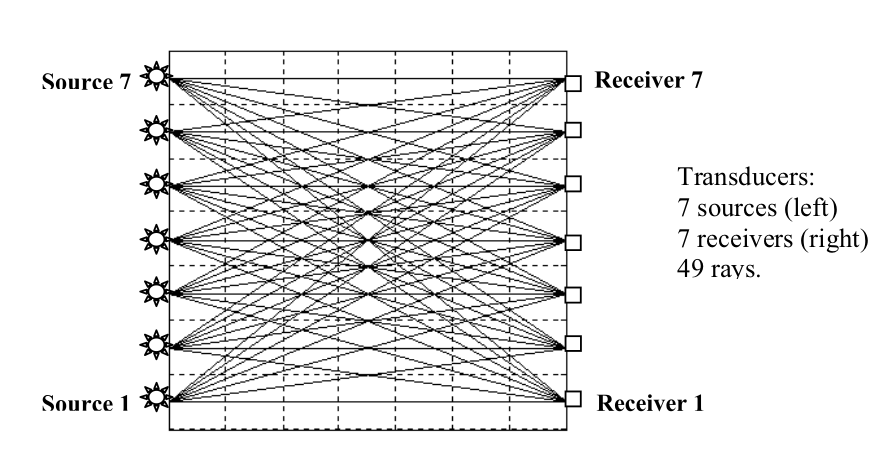
\includegraphics[scale=0.50]{Figuras/raios.png}
	\end{center}
	\caption{Traçado de raios. Discretização do espaço em 49 pixels. \textit{Cross-hole array}. \cite{RBGf1495}.}
	\label{raios}
\end{figure}

\begin{figure}[!hbtp]
	\begin{center}
		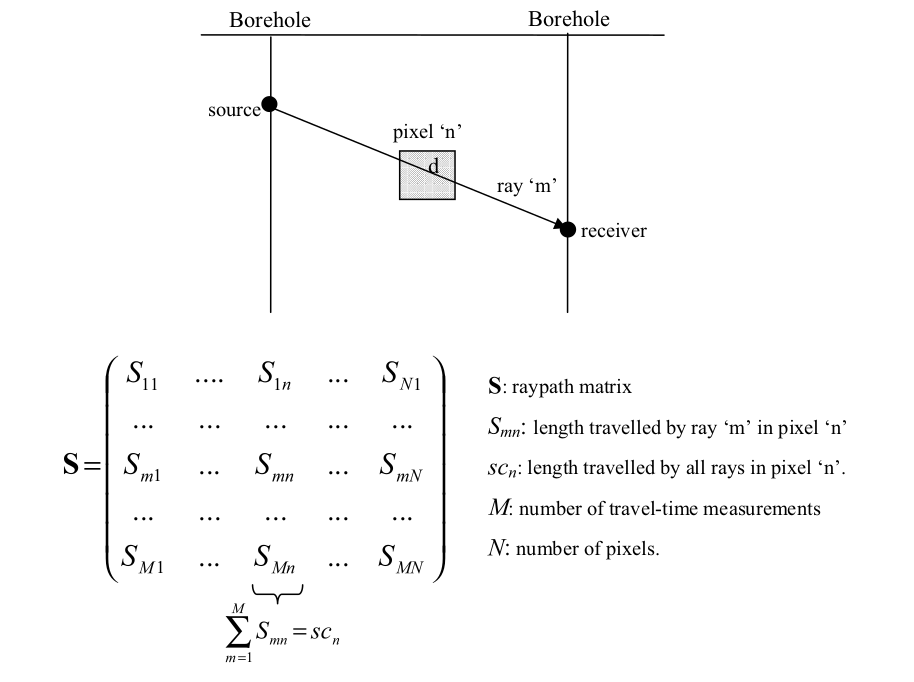
\includegraphics[scale=0.50]{Figuras/matriz_convergencia.png}
	\end{center}
	\caption{Matriz de percurso dos raios e significado de cobertura espacial. \cite{RBGf1495}.}
	\label{matriz_convergencia}
\end{figure}

\begin{figure}[!hbtp]
	\begin{center}
		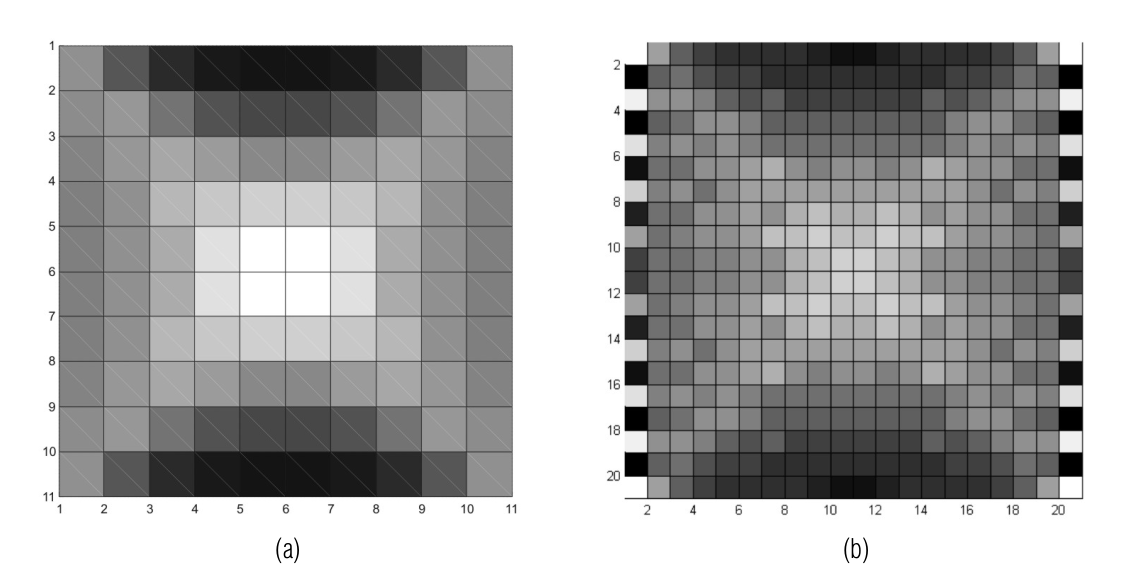
\includegraphics[scale=0.42]{Figuras/raios_convergencia.png}
	\end{center}
	\caption{Gráficos de cobertura espacial para pixels. (a) $10 \times 10$ pixels, (b) $20 \times 20$ pixels. \cite{RBGf1495}.}
	\label{raios_convergencia}
\end{figure} 

\begin{figure}[!hbtp]
	\begin{center}
		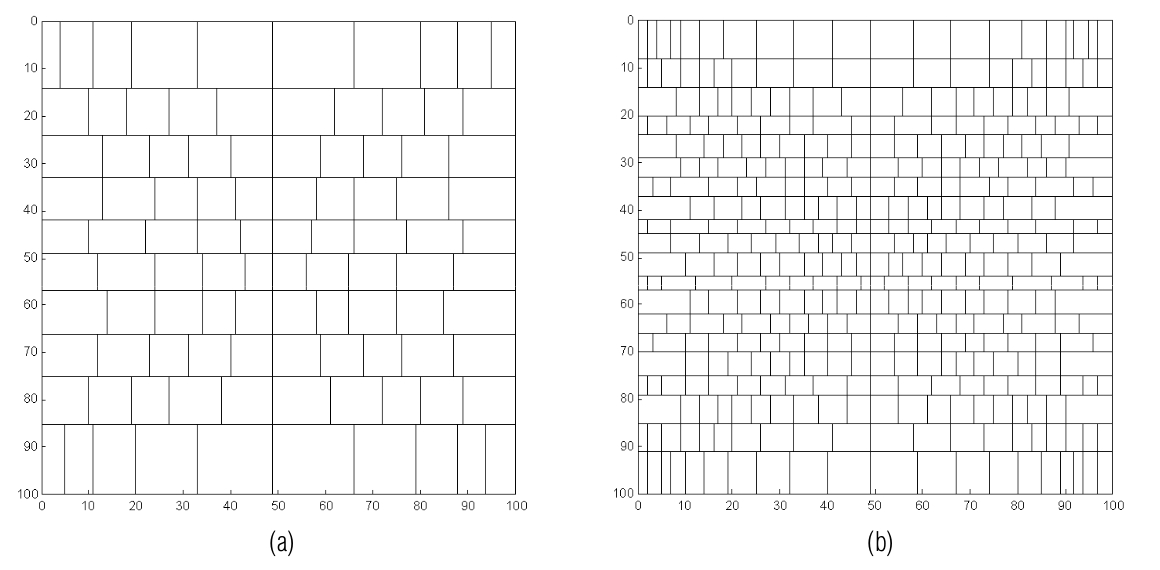
\includegraphics[scale=0.44]{Figuras/ipixel.png}
	\end{center}
	\caption{Gráficos de cobertura espacial Ipixel. (a) $10 \times 10$ ipixels, (b) $20 \times 20$ ipixels (calculados a partir de uma matriz de cobertura espacial  uniforme de base de $100 \times 100$ pixels). \cite{RBGf1495}.}
	\label{ipixel}
\end{figure} \newpage

%%%%%%%%%%%%%%%%%%%%%%%%%%%%%%%%%%%%%%%%%%%%%%

\subsection{Condicionamento de uma matriz}

Se houver um alto contraste entre os valores numéricos dos elementos dentro de uma matriz; é possível que a classificação calculada para ela tenha um número errôneo de linhas linearmente independente. Devido a isso, o número de condição $k$ é uma escolha melhor para estudar o condicionamento de uma matriz (ou seja, quão próximo está de uma matriz de classificação mais baixa) do que sua classificação (\citealp{strang1980linear}).

$k$ é definido como a razão entre os valores singulares com os valores absolutos máximos e mínimos (\citealp{computations1989johns}):

\begin{equation}\label{eq:k_equation}
k = \frac{max|\lambda _{i}|}{min |\lambda _{i}|}
\end{equation}

Uma matriz é dita mal condicionada se $k$ for muito grande. Geometricamente, os valores máximo e mínimo representam os eixos de uma elipse (\citealp{branham1990introduction}). Se a razão tende à unidade, a correlação é nula (independente) e se for muito grande, é quase perfeita (dependente) e portanto mal condicionada. Em outras palavras, mau condicionamento significa que o número de linhas ou colunas linearmente dependentes da matriz tende a aumentar. Isso significa que o número de equações/medidas diminui em relação ao número de incógnitas.

Por fim, os valores singulares dão uma indicação relacionada à confiança e à relação entre as medidas dos fenômenos. Valores pequenos sugerem informações limitadas sobre o parâmetro.

%%%%%%%%%%%%%%%%%%%%%%%%%%%%%%%%%%%%%%%%%%%%%%

\subsection{Regularização}

Problemas em tomografia geralmente são mal-postos, isto é, problemas que falham, seja na existência de soluções, na unicidade dessas soluções ou mesmo que a solução não depende continuamente dos dados (\citealp{tempopercurso}).  Sendo assim, são utilizadas frequentemente técnicas de regularização para dar estabilidade ao problema \citep{natterer2001mathematical}. Essas técnicas nos permitem solucionar não o problema original
mas sim, um problema similar, porém mais robusto em relação a erros nos dados.

Considere o problema de resolver $Ms = t$. Do ponto de vista matemático, no caso de modelos lineares, esses problemas mal-postos se devem geralmente ao fato da matriz $M$ possuir valores singulares nulos ou muito próximos de zero. Uma das formas de contornar isto seria acrescentar à matriz $M^{T}M$ um múltiplo da matriz identidade de tal maneira que essa nova matriz possua somente valores singulares positivos, porém distantes do zero. De fato, considerando $B = M^{T}M + \gamma I$, temos que se $\gamma \neq 0$, os autovalores de $B$ ficam diferentes de zero (positivos).

Feito isto, podemos definir a solução de mínimos quadrados amortecidos do sistema original por:

\begin{equation}\label{eq:regularization}
s' = (M^{T}M + \gamma I)^{-1}M^{T}t
\end{equation}

A escolha de um bom parâmetro $\gamma$ é fundamental nos problemas mal postos. O número $\gamma$ é chamado de parâmetro de regularização.

A não existência ou a perda de unicidade das soluções se devem ao fato de $t \notin Im(M)$ ou a não injetividade da transformação $M$, respectivamente. Nesses casos, a utilização da pseudo-inversa $M^{\dagger}$ é o mais conveniente. A técnica de regularização de Tikhonov consiste em obter certas transformações dadas denotadas por
$A_{\lambda}: \mathbb{R}^{n} \longrightarrow \mathbb{R}^{m}, \lambda > 0$, de tal forma,

\begin{equation}\label{eq:regularization_limite}
\lim_{\lambda \rightarrow 0} A_{\lambda}t = M^{\dagger}t
\end{equation}
onde $M^{\dagger}$ é a pseudo-inversa da matriz $M$.

Seja $t_{\epsilon} \in \mathbb{R}^{n}$ tal que $||t - t_{\epsilon}|| \leq \epsilon$. E seja $\lambda (\epsilon)$ tal que, quando $\epsilon \rightarrow 0$ 

\begin{equation}\label{eq:regularization_lim}
\lambda (\epsilon)  \rightarrow 0
\end{equation}
e

\begin{equation}\label{eq:regularization_codition}
||A_{\lambda (\epsilon)}||\epsilon \rightarrow 0
\end{equation}
assim,

\begin{equation}\label{eq:regularization_formulation}
||A_{\lambda (\epsilon)}t_{\epsilon} - M^{\dagger}t|| \leq ||A_{\lambda (\epsilon)}t_{\epsilon} - A_{\lambda (\epsilon)}t|| + ||A_{\lambda (\epsilon)}t - M^{\dagger}t|| \leq ||A_{\lambda (\epsilon)}|||t_{\epsilon} - t||| + ||A_{\lambda (\epsilon)}t - M^{\dagger}t|| \longrightarrow 0
\end{equation} \\

Logo, se $t_{\epsilon}$ está próximo do tempo de percurso $t$ então $A_{\lambda (\epsilon)}t_{\epsilon}$ está próximo
da solução aproximada $M^{\dagger}t$.

Como exemplo desse método consideremos a parada em um processo iterativo (\citealp{tempopercurso}). Seja então,

\begin{equation}\label{eq:regularization_formulation_exemplo}
s^{(k + 1)} = B_{k}s^{(k)} + C_{k}t
\end{equation}
um processo iterativo e assuma que $s^{(k)} \rightarrow M^{\dagger}t$. Para cada $\lambda > 0$, seja $k(\lambda)$ índice tal que $k(\lambda) \rightarrow \infty$ quando $\lambda \rightarrow 0$. Então afirmamos que $A_{\lambda}t = s^{(k(\lambda))}$ é uma regularização, pois

\begin{equation}\label{eq:regularization_formulation_exemplo2}
\lim_{\lambda \rightarrow 0} A_{\lambda}t = \lim_{\lambda \rightarrow 0} s^{(k(\lambda))} = M^{\dagger}t
\end{equation}
por hipótese.

Frequentemente no caso da tomografia por tempo de percurso a matriz $M$ (associada aos tempos de percurso dos raios sobre as células) tem posto deficiente ou é extremamente mal-condicionada. Isto leva naturalmente a necessidade de regularização.

%%%%%%%%%%%%%%%%%%%%%%%%%%%%%%%%%%%%%%%%

\clearpage

\section{Materiais e Métodos}

\subsection{Área de Estudo}

Para desenvolver a metodologia de tomografia sísmica para aquisição e processamento de dados em profundidades rasas (menores que 20 metros), inicialmente foi desenvolvido a técnica de maneira sintética e depois realizado uma aquisição em local com alvo conhecido, buscando otimizar os parâmetros de aquisição, e para calibrar as etapas de processamento. Tendo isso em vista, um alvo com dimensões e geometria conhecida foi instalado na área nos fundos do Observatório Sismológico no Campus Darcy Ribeiro da Universidade de Brasília (UnB), como pode ser observado na Figura~\ref{area_estudo} (página~\pageref{area_estudo}).
Como resultado, são gerados mapas de anomalias de velocidade que representa o alvo enterrado, e com isso, estabelecer um esquema de aquisição que permita resolver o alvo.

\begin{figure}[!hbtp]
	\begin{center}
		\includegraphics[scale=0.087]{Figuras/area-estudo.png}
	\end{center}
	\caption{Área de estudo nos fundos do Observatório Sismológico no Campus Darcy Ribeiro da Universidade de Brasília (UnB). A) Delimitando a área de estudo para a implantação do alvo. B) Imagem de satélite do Google Earth mostrando a localização da área de estudo (em vermelho).}
	\label{area_estudo}
\end{figure}
\newpage
%%%%%%%%%%%%%%%%%%%%%%%%%%%%%%%%%%%%%%%%%%%%%%%

\clearpage

\subsection{Frente teórica-computacional}

O trabalho foi elaborado em duas frentes: Uma teórico-computacional e outra experimental. Na frente teórico-computacional realizamos o desenvolvimento de rotinas computacionais para inversão dos dados de tempo de percurso (utilizando o tempo de chegada da onda direta). Utilizou-se de conceitos de inversão por mínimos quadrados com algum nível de regularização para controlar a ambiguidade do modelo de parâmetros (velocidade/vagarosidade). A estrutura computacional se necessária seria fornecida pelo Observatório Sismológico da UnB, e os programas/linguagens de programação utilizados são de código aberto (como Python, Matlab, Shellscript, etc). Elaborou-se modelos sintéticos com posição e propriedades físicas conhecidas das estruturas a serem simuladas. Os ajustes que por ventura sejam necessários foram incluídas no problema inverso, ou ainda, no esquema de aquisição. 

\begin{comment}
\begin{table}[!hbtp]
\centering
\caption{Parâmetros da aquisição sísmica realizada na barragem do Paranoá.}
\label{parametros_aquisicao_ativa}
\begin{tabular}{@{}lr@{}}
\toprule
\rowcolor[HTML]{FFFFFF} 
\multicolumn{1}{c}{\cellcolor[HTML]{FFFFFF}Parâmetros} & \multicolumn{1}{c}{\cellcolor[HTML]{FFFFFF}Valores} \\ \midrule
\rowcolor[HTML]{EFEFEF} 
Comprimento da linha                                   & 475 m                                               \\
\rowcolor[HTML]{FFFFFF} 
Espaçamento dos receptores                             & 5 m                                                 \\
\rowcolor[HTML]{EFEFEF} 
Espaçamento das fontes                                 & 10 m                                                \\
\rowcolor[HTML]{FFFFFF} 
Frequência geofones                                    & 14 Hz                                               \\
\rowcolor[HTML]{EFEFEF} 
Tipo de fonte                                          & Ativa (marreta)                                     \\
\rowcolor[HTML]{FFFFFF} 
Stacks                                                 & 3                                                   \\
\rowcolor[HTML]{EFEFEF} 
Janela temporal                                        & 1500 ms                                             \\
Taxa de amostragem                                     & 0.25 ms                                              \\ \bottomrule
\end{tabular}
\end{table}
\end{comment}

%%%%%%%%%%%%%%%%%%%%%%%%%%%%%%%%%%%%%%%%%%%%%%%%%%	

\subsubsection{Recursos computacionais}

Para a construção da rotina computacional, tanto para o desenvolvimento da etapa de gerar dados sintéticos com também para a etapa de processar os dados de campo para obter os mapas de tomografia sísmica, usamos a linguagem de programação Python. Ainda mais, é uma linguagem de programação de alto nível, ou seja, com sintaxe mais simplificada e próxima da linguagem humana, utilizada nas mais diversas aplicações, como desktop, web, servidores e ciência de dados e mais especificadamente com a biblioteca pyGIMLI, a utilização dessa linguagem atualmente encontra-se em crescimento no ramo da Geofísica no que diz respeito ao desenvolvimento de diversas rotinas de processamentos, utilizando-se dos conceitos dos métodos Geofísicos.


Por outro lado, pyGIMLi é uma biblioteca de código aberto para modelagem e inversão em Geofísica(\citealp{Ruecker2017}). A biblioteca orientada a objetos fornece gerenciamento para malhas estruturadas e não estruturadas em 2D e 3D. Uma tarefa principal do pyGIMli é realizar inversão. Vários tipos de regularização em malhas (1D, 2D, 3D) com disposição regular ou irregular estão disponíveis. Existe um controle flexível de todos os parâmetros de inversão. A estrutura de inversão padrão é baseada no método generalizado de Gauss-Newton. O pyGIMLi vem com vários operadores Geofísicos avançados, que podem ser usados diretamente para um determinado problema.

%%%%%%%%%%%%%%%%%%%%%%%%%%%%%%%%%%%%%%%%%%%%%%%

\subsubsection{pyGIMLi: Uma biblioteca de código aberto para modelagem e inversão em Geofísica}

Para que fosse possível o desenvolvimento do \textit{software}, as principais bibliotecas usadas foram o Matplotlib, Numpy e o pyGIMLi. O Matplotlib é um pacote de gráficos 2D usado em Python para desenvolvimento de aplicativos, scripts interativos e geração de imagens com qualidade de publicação em interfaces de usuário e sistemas operacionais (ver mais em \citealp{matplotlib}). No mundo Python, o NumPy é o pacote fundamental para computação científica. É uma biblioteca Python que fornece um objeto array multidimensional, vários objetos derivados (como arrays e matrizes) e uma variedade de rotinas para operações rápidas em arrays, incluindo matemática, lógica, manipulação de formas, classificação, seleção, I/O , transformadas discretas de Fourier, álgebra linear básica, operações estatísticas básicas e simulação aleatória (ver mais em \textit{\url{https://numpy.org/doc/1.22/}}).

Já o pyGIMLi, oferece uma vantagem distinta em que pode ser facilmente estendido por módulos compilados de C ou Fortran, por exemplo, permitindo aos usuários estender o código licenciado ou terceirizar partes demoradas em extensões computacionalmente eficientes. Realiza-se o uso dessa flexibilidade e implementa-se todas as partes sensíveis ao tempo de execução em uma biblioteca principal C++. As ligações completas do Python para essa biblioteca principal são complementadas por funcionalidades escritas em Python puro, oferecendo, assim, eficiência e flexibilidade para o rápido desenvolvimento de aplicativos robustos de modelagem e inversão. O componente de modelagem oferece gerenciamento de malha, bem como solucionadores de elementos finitos e volumes finitos em 1D, 2D e 3D. O componente de inversão é baseado em um algoritmo determinístico de Gauss-Newton e funciona com qualquer operador direto físico fornecido. Várias rotinas de pós-processamento são fornecidas para visualizar os resultados em 2D usando Matplotlib (\citealp{Ruecker2017}) e em 3D usando o software ParaView (Ayachit, 2015) ou Mayavi (Ramachandran e Varoquaux, 2011). 

%%%%%%%%%%%%%%%%%%%%%%%%%%%%%%%%%%%%%%%%%%%%%%%

\subsubsection{Estrutura do \emph{Software}}

\blindtext 
%
\blindtext 
%
\blindtext

%%%%%%%%%%%%%%%%%%%%%%%%%%%%%%%%%%%%%%%%%%%%%%%%

\subsection{Etapa experimental - Aquisição em local com alvo conhecido}

\blindtext 
%
\blindtext 
%
\blindtext

\begin{comment}
	\begin{itemize}
	
	\item Wavelet
	
	\end{itemize}
\end{comment}

\begin{comment}
\begin{table}[!hbtp]
\caption{Parâmetros utilizados nos modelos sintéticos de duas camadas.}
\centering
\label{parametros_gerais_modelos}
\begin{tabular}{@{}ll@{}}
\toprule
\multicolumn{1}{c}{Parâmetros} & \multicolumn{1}{c}{Valores} \\ \midrule
\rowcolor[HTML]{EFEFEF} 
Tempo de gravação          & 6, 12, 30, 60 e 120 s  \\
Número de fontes           & 100 \\
\rowcolor[HTML]{EFEFEF} 
Distância entre receptores & 1, 2, 4, 8 e 20 m      \\
Wavelet                    & $2^{a}$ Derivada Gaussiana   \\
\rowcolor[HTML]{EFEFEF} 
Frequência máxima          & 30 Hz                  \\
Frequência de pico         & 15 Hz                  \\
\rowcolor[HTML]{EFEFEF} 
Discretização (dx e dz)    & 1 m                    \\
Amostragem (dt)            & 0.009 s                \\ \bottomrule
\end{tabular}
\end{table}
\end{comment}


\clearpage

%%%%%%%%%%%%%%%%%%%%%%%%%%%%%%%%%%%%%%%%%%%%%%%%%%%%%

\section{Resultados e Discussão}
\label{ResultadosDiscussao}

\subsection{Dados sintéticos - Estudos de casos}

\blindtext 
%
\blindtext 
%
\blindtext

\begin{comment}
\begin{table}[!hbtp]
\caption{Velocidades da onda P características de diferentes materiais geológicos. Modificado de \cite{oliveira1998geologia}.}
\centering
\label{tabela_vp}
\begin{tabular}{@{}ll@{}}
\toprule
$V_{p}$ (m/s)                         & Material                                                                                                                                          \\ \midrule
\rowcolor[HTML]{EFEFEF} 
{\color[HTML]{000000} 200 - 400} & {\color[HTML]{000000} Solos, sedimentos inconsolidados}                                                                                           \\
400 - 1400                       & Argilas/areias inconsolidadas                                                                                                                     \\
\rowcolor[HTML]{EFEFEF} 
1400 - 1800                      & \begin{tabular}[c]{@{}l@{}}Areias saturadas, argila compactadas, \\ rochas muito alteradas\end{tabular}                                           \\
1800 - 2400                      & \begin{tabular}[c]{@{}l@{}}Sedimentos consolidados/saturados, \\ rochas ígneas/metamórficas, rochas\\ alteradas, arenitos, folhelhos\end{tabular} \\
\rowcolor[HTML]{EFEFEF} 
2400 - 3700                      & \begin{tabular}[c]{@{}l@{}}Arenitos, folhelhos, rochas ígneas/\\ metamórficas alteradas\end{tabular}                                              \\ \bottomrule
\end{tabular}
\end{table}
\end{comment}



\clearpage 

%%%%%%%%%%%%%%%%%%%%%%%%%%%%%%%%%%%%%%%%%%%%%%%%%%

\subsection{Dados de campo - Processamento e inversão dos dados sísmicos}

\blindtext 
%
\blindtext 
%
\blindtext

\clearpage

%%%%%%%%%%%%%%%%%%%%%%%%%%%%%%%%%%%%%%%%%%%%%%%%%%%

\section{Conclusões}

\blindtext 
%
\blindtext 
%
\blindtext


\clearpage

%%%%%%%%%%%%%%%%%%%%%%%%%%%%%%%%%%%%%%%%%%%%%%%%%%%%%

\bibliographystyle{seg}
\bibliography{Referencias}


\clearpage

%%%%%%%%%%%%%%%%%%%%%%%%%%%%%%%%%%%%%%%%%%%%%%%%%%%%%

\appendix
\section{Código do \emph{software}}
\label{apendice_scr}

\begin{comment}
\begin{lstlisting}[language=Bash, caption=Exemplo de script utilizado para gerar o modelo de duas camadas]

#!/bin/bash
#PBS -l nodes=1:ppn=2
#PBS -N InterfModeling
#PBS -V

#rm *.su *.bin *.txt *.eps nep *.ascii

export PATH=../../utils:$PATH

export OMP_NUM_THREADS=8

########################################
########################################
########## MODELO GEOLOGICO ############
########################################
########################################

makewave file_out=wavelet.su dt=0.0001 nt=1024 fp=15 shift=1 w=g2 verbose=1

makemod file_base=modelo.su \
cp0=400 ro0=1800 cs0=200 sizex=1200 sizez=100 \
dx=1 dz=1 orig=0,0 \
intt=def poly=0 cp=4500 ro=2100 cs=1900 \
x=0,1200 z=50,50 gradcp=0 grad=0 \
verbose=4

export filecp=modelo_cp.su
export filecs=modelo_cs.su
export filero=modelo_ro.su

suximage < modelo_cp.su legend=1 title="Modelo geologico" & 

########################################
########################################
############### ATIVO ##################
########################################
########################################

rec=rec_ativo.su
snap=snap_ativo.su

../fdelmodc \
	file_cp=$filecp file_cs=$filecs file_den=$filero \
	ischeme=1 iorder=4 \
	file_src=wavelet.su verbose=4 \
	file_rcv=$rec \
	file_snap=$snap \
	xrcv1=1 xrcv2=1200 dxrcv=1 \
	zrcv1=0 zrcv2=0 \
	rec_type_vx=1 rec_type_vz=1 rec_int_vx=1 rec_int_vz=1 \
	dtrcv=0.009 fmax=30 dt=0.0001 \
	xsrc1=600 xsrc2=600 zsrc1=0 zsrc2=0 nshot=1 plane_wave=0 amplitude=0  \
	src_type=1 tmod=2.0 tlength=$tmod tsrc1=0 tsrc2=$tmod \
	ntaper=45 rec_ntsam=16384 \
	left=4 right=4 bottom=4 top=4 

suximage < rec_ativo_rvz.su title="Gravacao de uma fonte ativa" & 

########################################
########################################
############## PASSIVO #################
########################################
########################################

itmin=0

suwind itmin=$itmin < $filecp | sushw key=f1 a=0.5 > vel_cp.su
suwind itmin=$itmin < $filecs | sushw key=f1 a=0.5 > vel_cs.su
suwind itmin=$itmin < $filero | sushw key=f1 a=0.5 > vel_ro.su

rec=rec.su
snap=snap.su
tmod=6.0

../fdelmodc \
	file_cp=vel_cp.su file_cs=vel_cs.su file_den=vel_ro.su \
	ischeme=1 iorder=4 \
	file_src=wavelet.su verbose=4 \
	file_rcv=$rec \
	file_snap=$snap \
	xrcv1=1 xrcv2=1200 dxrcv=1 \
	zrcv1=0 zrcv2=0 \
	rec_type_vx=1 rec_type_vz=1 rec_type_p=1 \
	rec_int_vx=1 rec_int_vz=1 rec_int_p=1 \
	dtrcv=0.009 fmax=30 dt=0.0001 \
	xsrc1=1 xsrc2=1199 zsrc1=1 zsrc2=99 nsrc=100 nshot=1 plane_wave=0 \
	src_type=1 tmod=$tmod tlength=$tmod \
	tsrc1=0 tsrc2=$tmod amplitude=0 wav_random=1 \
	ntaper=45 src_random=1 rec_ntsam=16384 \
	tsnap1=0 tsnap2=$tmod dtsnap=1  \
	sna_type_p=1 sna_type_vz=4 \
	left=4 right=4 top=4 bottom=4

suximage < rec_rvz.su perc=99 "Registro Vz " &  

########################################
########################################
######### Fontes e Receptores ##########
########################################
########################################

suop2 SrcRecPositions.su $filecp w1=7000 w2=1 op=sum |\
sugain nclip=1 > SrcModel.su

suximage < SrcModel.su & # Fontes e Receptores sobrepostos no modelo geologico

########################################
########################################
###### Auto-correlacao das fontes ######
########################################
########################################

fconv file_in1=src_nwav.su auto=1 shift=1 mode=cor1 | \
	sugain qbal=1 | \
	supswigp x1beg=-1 x1end=1 d2num=10 hbox=4 wbox=6 \
	labelsize=10 label2='Numero de Fonte' label1='Tempo (s)' \
	titlesize=-1 fill=0 > src_nwav_autoCorr_Norm.eps

gv src_nwav_autoCorr_Norm.eps & # Auto-correlacao das fontes

########################################
########################################
############# Correlacoes ##############
########################################
########################################

shot=rec_rvz.su
base=`echo $shot | awk 'BEGIN { FS = ".su" } ; { print $1 }'`
echo $base

tmax=2.0

ntraces=`surange < $shot | grep traces| awk '{print $1 }'`
echo $ntraces
middle=$(echo "scale=0 ; ($ntraces+1)/2"| bc -l)
echo $middle

suwind key=tracl min=$middle max=$middle < $shot > middleTrace.su

fconv verbose=1 file_in1=$shot file_in2=middleTrace.su mode=cor1 shift=1 > corr.su

ns=`surange < corr.su | grep ns | awk '{print $2 }'`

odd=$(( ns % 2))
if [[ $odd == 1 ]]; then
  ns2=$(echo "scale=0; ($ns-1)/2"| bc -l)
  ns=$(echo "scale=0; $ns-1"| bc -l)
else
  ns2=$(echo "scale=0; ($ns)/2"| bc -l)
fi

echo $ns $odd
echo $ns2

suwind < corr.su itmin=0 itmax=$ns2 | suflip flip=3 > noncausal.su
suwind < corr.su itmin=$ns2 itmax=$ns > causal.su

tot=$(echo "scale=0; ($tmod) + 0.01"| bc -l)
dxrcv=1

susum causal.su noncausal.su | suwind s=1 j=1 tmax=$tmax f1=0.0 |\
sushw key=f1,delrt,d2 a=0.0,0.0,$dxrcv > ${base}_add.su 

suximage < ${base}_add.su perc=99 title="Imagem recuperada apos a interferometria" & 

########################################
########################################
########### Figuras Tracos #############
########################################
########################################

psgraph < srcTimeLengthN\=60001.bin n1=60001 \
    labelsize=12 d1=0.0001 style=normal linecolor=blue \
    label1="start time (s)" label2="source duration (s)" \
    d1num=1 d2num=1 wbox=8 hbox=4 x1end=$tmod x2end=$tmod > srcTimeLength.eps

gv srcTimeLength.eps & # Ativacao das fontes

supswigp < src_nwav.su \
	labelsize=10 label1='Tempo (s)' label2='Numero da Fonte' x1end=6 \
	d2=1 d2num=10 hbox=4 wbox=6 fill=0 \
	titlesize=-1 > src_nwav.eps

gv src_nwav.eps & # Tracos sismicos das fontes

traclrange=`surange < src_nwav.su | grep tracl` 
trace1=`echo $traclrange | cut -f2 -d" " `
trace2=`echo $traclrange | cut -f3 -d" " `

echo "tracerange = $trace1 $trace2"

for (( trace = $trace1; trace<=$trace2; trace+=1 )) do
	echo $trace
	suwind < src_nwav.su key=tracl min=$trace max=$trace  > trace.su 
	fconv file_in1=src_nwav.su file_in2=trace.su file_out=cross.su mode=cor1 fmax=31 fmin=0
	suwind < cross.su itmax=0 itmin=0 | sustrip >> corr2d.bin
done

suaddhead < corr2d.bin n1=100 | sugain pbal=1 dt=1 | suop op=abs | \
	sugain scale=0.1005 dt=1 | \
	supsimage  legend=1 hbox=3 wbox=3 \
	titlesize=-1 labelsize=10 label1="Numero da Fonte" label2="Numero da Fonte" \
	d1=1 f1=1 f1num=0 d1num=20 d2num=20 > cross2d.eps

gv cross2d.eps & # Fator correlacao

echo "Fim da Modelagem"

exit;

\end{lstlisting}
\end{comment}


\end{document}




